\documentclass[11pt,a4paper]{article}

\usepackage{amsmath,amsfonts,graphicx,psfrag,color}
\usepackage{algorithm}
\usepackage[textsize=small]{todonotes}
\usepackage{booktabs}
\usepackage{subcaption}
\newtheorem{definition}{Definition}

\setlength{\parindent}{0ex}

\topmargin=-0.5in
\oddsidemargin=0in
\evensidemargin=0in
\textwidth=6.5in
\textheight=9.5in

\newcommand{\note}[1]{\par\medskip\textsc{\textbf{NOTE:} {#1}}\par\medskip}

\title{Bayesian parameter estimation for quantitative
systems pharmacology}
\author{Tom Lowe, Colin Gillespie, Andrew Golightly}
\date{School of Mathematics, Statistics and Physics, Newcastle University,\\
  Newcastle upon Tyne, NE1 7RU, UK}
  
\begin{document}
\maketitle

\section{Introduction and overview}
\label{sec:intro}

This report concerns the modelling of the growth of tumours implanted in mice, and the estimation of parameters governing these models. Previous studies such as \cite{yates14} have focused on frequentist parameter estimation. However, a frequentist approach assumes a set of unknown but fixed parameters, whereas here the focus is on Bayesian parameter estimation, which takes into account the uncertainty about the parameters being estimated. Furthermore, the report looks at random effects models, whereby the parameters of the model may vary among individual mice, yet come from a common distribution.

There are a range of different models that can be used for the modelling of tumour growth; a comparison of many of these can be found in \cite{evans17}. This report looks at the Warwick model, a simplified version of the tumour growth model proposed in \cite{yates14}. This models the tumour as an expanding sphere consisting of a proliferating shell surrounding a core which does not exhibit cell replication. The volume of this tumour, $V_t$, evolves over time according to 
\[
\frac{dV_t}{dt} = kV_t\left(1-\left(1-\frac{r_d}{\left(\frac{3V_t}{4 \pi} \right)^{1/3}}\right)^3\right),
\]
where $k$ is the growth rate of the proliferating shell, and $r_d$ is its thickness (assumed to be constant). The model requires an initial condition, $V_0$ (the volume at time 0) to complete the specification. The relationship between the volume and radius of the tumour, $r_t$ is
\[
V_t = \frac{4}{3} \pi r_t^3,
\]
so the model can be written as
\[
\frac{dV_t}{dt} = kV_t\left(1-\left(1-\frac{r_d}{r_t}\right)^3\right).
\]
Thus we can see that the model represents exponential growth, weighted by the ratio of the shell thickness and the overall diameter of the tumour - as the tumour increases in volume, $r_d/r_t$ will decrease, thus decreasing the term weighting $kV_t$, and slowing the growth of the tumour. 

This interpretation of the model is useful in explaining observed behaviour of tumours in a mechanistic way, however the model does have its limitations. Firstly, the model does not require $r_d \leq r_t$, meaning that scenarios where the thickness of the proliferating shell is larger than the entire radius of the tumour including the shell are plausible (in practice the model is replaced with the exponential model until it grows to a point where $r_t \geq r_d$, but this is still problematic in terms of physical interpretation of the model). Secondly, there are no constraints on the relationship between the growth rate and the thickness of the shell, meaning that increasing one parameter and decreasing the other in the right way can lead to almost identical behaviour in the evolution of the system, thus leading to identifiability problems.
\begin{figure}
\centering
\includegraphics[width=0.5\textwidth, angle = 270]{k_rd_histograms.eps}
\caption{Histograms highlighting the differences in magnitude between maximum likelihood estimates of $k$ and $r_d$.}
\label{fig:hist}
\end{figure}
Both of these problems can be seen in Figure \ref{fig:hist}. The data in this figure are from the Warwick model being fit to the growth of 212 different tumours from \cite{Gao15}. The parameters for each of these fits have been inferred using maximum likelihood estimation techniques, and the (base 10) logarithm of these estimates have been plotted in histograms, so that each unit on the $x$-axis corresponds to an order of magnitude difference in the estimates of the parameters. Firstly, the largest estimate of $r_d$ in this dataset is $119.28mm$, which corresponds to a tumour with an initial volume of $216.67mm^3$, and therefore an initial radius of $3.73mm$, over thirty times smaller than the thickness of the proliferating shell. Secondly, we can see from the figure that the estimates for each of these parameters vary by over 10 orders of magnitude, and even discounting the three extreme observations on the left of the histograms, estimates still differ by 6 orders of magnitude. These differences are very large, particularly when the initial volume of these tumours are all of the same order of magnitude, and makes it difficult to draw conclusions about the parameters for a general population of tumours.
\begin{figure}
\centering
\includegraphics[width=0.5\textwidth, angle=270]{rd_v_k.eps}
\caption{A plot of $r_d$ against $k$, viewed on the log scale.}
\label{fig:rd_v_k}
\end{figure}
\begin{figure}
\centering
\includegraphics[width=0.5\textwidth, angle=270]{rd_x_k.eps}
\caption{A plot of $r_d$ multiplied by $K$, viewed on the log scale.}
\label{fig:rd_x_k}
\end{figure}

If we plot the estimates of the two parameters against each other, as in Figure \ref{fig:rd_v_k}, we can see the strong negative correlation between them. However, plotting the product of the estimates of the two parameters, as in Figure \ref{fig:rd_x_k}, we see that aside from the three outliers, the products all have a very similar order of magnitude. This implies that our estimates of the parameters may be subject to these identifiability issues.

To circumvent this problem, the model can be reparametrized. Let $\alpha = k \times r_d$. If one of $k$ or $r_d$ is fixed, $\alpha$ can then be estimated to determine the relationship between the two other parameters. Here, $r_d$ shall be fixed at
\[
r_d = \left(\frac{3V_0}{4 \pi}\right)^{1/3},
\]
the radius of the tumour at time 0. This will also address the issue of $r_d$ being larger than $r_t$, as fixing $r_d$ at this value will ensure that this does not occur.

\section{Applications to mouse tumour growth}
\label{sec:results}

In this sections, we fit the random effects model given in Appendix \ref{appendix} to data from a single treatment group (Section \ref{subsec:app1}) before considering multiple treatment groups (Section \ref{subsec:app2}).

\subsection{Application to a single treatment group}
\label{subsec:app1}

Data were provided from AstraZeneca for tumour growth in five xenografted mice. The volume of the tumour was recorded on the day of initial establishment of the tumour and then at 3, 7, 10, 14, 17, 21, 24 and 28 days afterwards. We assumed the tumours evolved according to the Warwick model, with either additive or multiplicative Gaussian noise of mean 0 and standard deviation $\sigma_i$ (which may differ between individuals). We fitted a Bayesian random effects model for each of these noise assumptions using a Metropolis-Hastings scheme. Details of the full model and the scheme can be found in Appendix \ref{appendix}.
\begin{figure}
\centering
\includegraphics[width=0.5\textwidth, angle=270]{alphaBarDensity.eps}
\caption{Marginal posterior density plot for the population median of $\alpha$, under both the additive and multiplicative noise schemes.}
\label{fig:alphaBarDensity}
\end{figure}
%\begin{figure}
%\centering
%\includegraphics[width=0.5\textwidth]{tauDensity.jpg}
%\caption{Marginal posterior density plot for $\tau$, the population precision of $\alpha$}
%\label{fig:tauDensity}
%\end{figure}
Figure \ref{fig:alphaBarDensity} shows the marginal posterior distribution of the population average of the $\alpha_i$, under both additive and multiplicative noise schemes, noting that there is very little difference between these posterior distributions. We emphasise that our approach provides a quantification of the uncertainty in all parameter values.
\begin{table}
\centering
\begin{tabular}[c]{|l|c c c|}
\hline
Mouse & $\alpha_i$ & $V_0^i$ & $\sigma_i$ \\
\hline
1 & 0.0257 (0.0013) & 0.001815 (0.0023) & 0.0337 (0.0102) \\
2 & 0.0295 (0.0017) & 0.000454 (0.0012) & 0.0310 (0.0092) \\
3 & 0.0346 (0.0022) & 0.000595 (0.0056) & 0.3827 (0.1218) \\
4 & 0.0323 (0.0019) & 0.000576 (0.0018) & 0.1479 (0.0445) \\
5 & 0.0269 (0.0015) & 0.002529 (0.0053) & 0.1363 (0.0418) \\
\hline
\end{tabular} 
\caption{Marginal posterior means (standard deviations in parentheses) for $\alpha_i$, $V_0^i$ and $\sigma_i$ for each of the five mice under the assumption of additive noise.}
\label{tab:summaryAdd}
\end{table}
\begin{table}
\centering
\begin{tabular}[c]{|l|c c c|}
\hline
Mouse & $\alpha_i$ & $V_0^i$ & $\sigma_i$ \\
\hline
1 & 0.0263 (0.0018) & 0.000681 (0.0005) & 0.6311 (0.2192) \\
2 & 0.0322 (0.0016) & 0.001763 (0.0007) & 0.4157 (0.1316) \\
3 & 0.0334 (0.0021) & 0.001662 (0.0013) & 0.5951 (0.1971) \\
4 & 0.0309 (0.0020) & 0.008850 (0.0037) & 0.5371 (0.1641) \\
5 & 0.0268 (0.0025) & 0.007688 (0.0050) & 0.9117 (0.2974) \\
\hline
\end{tabular} 
\caption{Marginal posterior means (standard deviations in parentheses) for $\alpha_i$, $V_0^i$ and $\sigma_i$ for each of the five mice under the assumption of multiplicative noise.}
\label{tab:summaryMult}
\end{table}
Table \ref{tab:summaryAdd} shows the posterior means for the parameters for all five mice under the assumption of additive noise, and Table \ref{tab:summaryMult} shows the same means and standard deviations under the assumptions of multiplicative noise. In both cases, our individual estimates of $\alpha_i$ agree with our population average distribution. The standard deviations of $V_0^i$ estimates tend to be smaller in the multiplicative scheme, and the estimates of $\sigma_i$ are quite different between the two schemes, which is to be expected as $\sigma_i$ has a different interpretation in the different schemes.
\begin{figure}
\centering
\includegraphics[width=0.6\textwidth]{SolsMouse1withMean.pdf}
\caption{1000 solutions of $dV_t/dt$ for mouse 1 for both additive and multplicative schemes, with parameters from the MCMC scheme. Darker areas contain more posterior density. Solutions from posterior means of $\alpha_1$ and $V_0^1$ in dashed line.}
\label{fig:solutions}
\end{figure}
Figure \ref{fig:solutions} shows 1000 solutions of the ordinary differential equation (ODE) $dV_t/dt$ for mouse 1 (similar plots were produced for the other mice) using posterior samples of $\alpha_1$ (which is used to deterine $k_1$), $V_0^1$, and fixing $r_{d,1}$ as described in section \ref{sec:intro}. The data points have been overlaid onto the plot. The grey lines can be thought of as samples from from the posterior predictive distribution of the underlying process. We see that the data are reasonably consistent with these samples in both the additive and multiplicative schemes, suggesting that the ODE model provides a reasonable fit to the data. The error in the additive noise scheme stays reasonably constant throughout the solution (as is to be expected), whereas the error in the multiplicative noise scheme grows as the solution grows, so the solution curves are very concentrated around the first few observations, and grow more diffuse as time increases. This leads to observations that are encompassed within the solution curves of the multiplicative scheme that are not within those of the additive scheme. In addition, the solution curve using the posterior means of $\alpha_1$ and $V_0^1$ was calculated for each scheme and overlaid with a dashed line. It would appear that using the marginal posterior mean parameter values from the multiplicative model lead to an ODE solution that fits the data better than typical solutions from the additive model.

%Our current work involves allowing the remaining parameters to be random effects, and comparing this treatment group of five mice to different treatment groups via the posterior distributions of the population level parameters, to determine possible fixed effects between groups.

\subsection{Application to multiple treatment groups}
\label{subsec:app2}

Data were taken from \cite{Gao15} consisting of tumour growth in 212 mice, which were implanted with one of six different tumour types: gastric cancer (GC), colorectal cancer (CRC), breast carcinoma (BRCA), pancreatic ductal adenocarcinoma (PDAC), non-small lung carcinoma (NSCLC), or cutaneous melanoma (CM). Tumor volume was measured approximately twice weekly, although different mice were measured on different days and for different amounts of time. In this scenario we assumed multiplicative noise, and grouped the mice into groups according to the type of tumour they had been implanted with. We then fitted a Bayesian random effects model using a Metropolis-Hastings scheme for each of these tumour types, so that the fixed effects of each treatment group can be compared by comparing the output of each scheme.
\begin{figure}
\centering
\includegraphics[width=0.5\textwidth]{alphaBarMeans.pdf}
\caption{Marginal posterior means and one standard deviation for $\bar{\alpha}$, for each of the six tumour types.}
\label{fig:alphaBarMeans}
\end{figure}
\begin{figure}
\centering
\includegraphics[width=0.5\textwidth]{V0BarMeans.pdf}
\caption{Marginal posterior means and one standard deviation for $\bar{V_0}$, for each of the six tumour types.}
\label{fig:V0BarMeans}
\end{figure}
Figures \ref{fig:alphaBarMeans} and \ref{fig:V0BarMeans} show the marginal posterior means, with an error bar of one standard deviation, for $\bar{\alpha}$ and $\bar{V_0}$ respectively, for each of the six tumour types. From Figure \ref{fig:alphaBarMeans}, we see that the CM tumour appears to grow significantly quicker than the others, and mice with the NSCLC tumour have the largest variance in $\alpha$ values. From figure \ref{fig:V0BarMeans}, we see that the two tumour types with the largest $\bar{\alpha}$ parameter also have the two smallest $\bar{V_0}$ parameters. This means that on average, mice with these two tumour types will have had smaller tumours at time 0. Because the $V_0$ parameter is deterministically related to the $r_d$ parameter in our parameterization, this means that mice with these tumours must also have had the smallest values of the $r_d$ parameter, and thus the growth rate $k$ would have had to be even larger to make $\alpha = k \times r_d$ greater than the other tumour types.
\begin{figure}
\centering
\includegraphics[width=0.6\textwidth]{GC_sols.pdf}
\caption{1000 solutions of $dV_t/dt$ for a mouse with a GC tumour, with parameters from the MCMC scheme. Darker areas contain more posterior density. Solutions from posterior means of $\alpha$ and $V_0$ in dashed line, with solutions from frequentist estimates of $k$, $V_0$ and $r_d$ in dotted line.}
\label{fig:GC_sols}
\end{figure}
\\
As in sections \ref{subsec:app1}, in Figure \ref{fig:GC_sols} we have plotted 1000 solutions of $dV_t/dt$ using posterior samples of $\alpha$ and $V_0$, for a mouse with a GC tumour. Barring one outlier where our tumour volume appears to decrease, our solutions seem to fit the observed data quite well. We have overlaid the solution using the posterior means of the parameters from our Bayesian analysis, and also the solution using the frequentist maximum likelihood techniques, as illustrated in section \ref{sec:intro}, and the fits appear to be very similar. The parameters inferred using the frequentist techniques were $k$, $V_0$ and $r_d$, and the parameters inferred using Bayesian techniques were $\alpha$ and $V_0$, but using the fact that $\alpha = k \times r_d$, and that the parameterization used in the Bayesian analysis fixed $r_d = \left(\frac{3V_0}{4 \pi}\right)^{1/3}$, we can compare the two sets of parameters, which are seen in Table \ref{tab:freq_v_bayes}.
\begin{table}
\centering
\begin{tabular}[c]{|l|c|c|c|c|}
\hline
 & $V_0$ & $r_d$ & $k$ &  $\alpha$ \\
\hline
Bayesian & 217.87 & 3.73 & 0.056 & 0.21 \\
Frequentist & 209.48 & 52.4 & 0.058 & 3.05 \\
\hline
\end{tabular} 
\caption{Comparison of Bayesian and frequentist estimates for $V_0$, $r_d$, $k$ and $\alpha$.}
\label{tab:freq_v_bayes}
\end{table}
We can see that the growth rate $k$ is very similar in both estimates, and the initial volume $V_0$ is fairly similar (although the Bayesian estimate is closer to the observed value). The main difference between the two estimates is the $r_d$ value (which is in turn skewing the $\alpha$ value). The frequentist estimate for $r_d$ is $52.4mm$, a shell thickness which corresponds to the entire diameter of a tumour with a volume of $V_t = 602800mm^3$, much larger than the largest observed tumour volume of $V_t=1710mm^3$, which equates to a radius of $r_t=7.42mm$. This again highlights the issues of physical interpretation of the original parameterization of the Warwick model, and we also note that in this case the Warwick model has essentially been replaced with the simple exponential model here for the entire solution.

\section{Conclusions}
\label{sec:conc}

In this report we have identified issues with a currently used model for tumour growth, reparameterized the model to alleviate these problems, and used the reparameterized model within a Bayesian random effects framework to estimate the parameters governing the model, and investigated the assumption of both additive and multiplicative Gaussian noise within this framework. We have applied this to two scenarios, a simple scenario with five mice implanted with the same tumour type and measured at regular intervals for regular ammounts of time, and a more complex scenario featuring 212 mice implanted with one of six different tumour types, measured at irregular intervals for irregular lengths of time. We found that the solutions from our posterior distributions fit our observed data well, and the assumption of multiplicative noise gave a more realistic fit than the assumption of additive noise. We also found that we could compare several different tumour types, or in a more general sense `treatment groups', by running seperate inference schemes for each group and comparing the output.

Future work in this area could include refining the reparameterization of the model, using biological as well as mathematical arguments, and eliciting and utilising expert prior information, which may enable relaxation of the constraints on parameters within the model. Another useful addition to the model would be that of a treatment effect, as all tumours studied here were untreated. Another way to approach the problem could be to use stochastic differential equations, as they account for intrinsic stochastisity within the solution, rather than simply modelling it as observation noise. However, inference using stochastic differential equations is challenging, as it requires integration over additional uncertainty.

\appendix

\section{Bayesian random effects model}
\label{appendix}

Suppose we have $M$ individuals (mice). According to the Warwick model, for each individual $i$, $i=1,\ldots, M$, our volume $V_t^i$ evolves according to
\[
\frac{dV_t^i}{dt} = k_iV_t^i\left(1-\left(1-\frac{r_{d,i}}{\left(\frac{3V_t^i}{4 \pi} \right)^{1/3}}\right)^3\right).
\] 
We have observations at discrete times, $Y_t^i$. We can assume that our observations are subject to either additive or multiplicative Gaussian noise. Assuming additive noise leads to the observation equation
\[
Y_t^i = V_t^i + \varepsilon_t^i, \quad \varepsilon_t^i \sim N(0, \sigma_i^2), \quad i = 1, \ldots, M,
\]
whereas assuming multiplicative noise leads to the observation equation
\[
\log(Y_t^i) = \log(V_t^i) + \varepsilon_t^i, \quad \varepsilon_t^i \sim N(0, \sigma_i^2), \quad i = 1, \ldots, M.
\]
In either case, inference proceeds in an identical manner. For each individual we have three parameters to infer: $V_0^i$, $\sigma_i$, and $\alpha_i = r_{d,i} \times k_i$. Denote the vector of these parameters to be $\boldsymbol{\theta}_i$. As these parameters are all strictly positive, we shall work with the natural logarithms of these parameters, and so use a vague Gaussian prior of $N(0, 10^2)$ for all $V_0^i$ and $\sigma_i$ parameters. Assuming that the $\alpha_i$ parameters are all individual realisations from a population distribution, we incorporate these random effects by introducing a hierarchichal prior for the $\alpha_i$, such that
\[
\log(\alpha_i) \sim N(\bar{\alpha}, 1/\tau_\alpha), \quad i = 1, \ldots, M.
\]
We introduce semi-conjugate hyperpriors for $\bar{\alpha}$ and $\tau_\alpha$, that is,
\begin{align*}
\bar{\alpha} & \sim N(b, 1/d), \\
\tau_\alpha & \sim Ga(g,h). \\
\end{align*}

Given data $\boldsymbol{y} = (\boldsymbol{y}^1, \ldots, \boldsymbol{y}^M)^T$, where $\boldsymbol{y}^i = (y_{t_1}^i, \ldots, y_{t_n}^i)^T$ for $n$ time points, Bayesian inference proceeds via the posterior distribution
\begin{equation}
\pi(\boldsymbol{\theta}_1, \ldots, \boldsymbol{\theta}_M|\boldsymbol{y}) = \prod_{i=1}^M\pi(\boldsymbol{\theta}_i|\boldsymbol{y}) \propto \pi(\boldsymbol{V}_0) \pi(\boldsymbol{\sigma}) \prod_{i=1}^M \left[ \pi(\alpha_i|\bar{\alpha}, \tau_\alpha) \pi(\boldsymbol{y}^i|\boldsymbol{\theta}_i) \right],
\label{eq:post}
\end{equation}
where
\[
\pi(\boldsymbol{V}_0) = \prod_{i=1}^M\pi(V_0^i), \quad \pi(\boldsymbol{\sigma}) = \prod_{i=1}^M\pi(\sigma_i),
\]
and
\[
\pi(\boldsymbol{y}^i|\boldsymbol{\theta}_i) = \prod_{j=1}^n N(y_{t_j}^i; V_{t_j}^i, \sigma_i^2).
\]
Although the posterior (\ref{eq:post}) will be intractable, inference may proceed via a Gibbs sampler, with draws from the following full conditional distributions (FCDs)
\begin{enumerate}
\item $\pi(\bar{\alpha}|\tau_\alpha, \alpha_1,\ldots,\alpha_M)$

\item $\pi(\tau_\alpha|\bar{\alpha}, \alpha_1,\ldots,\alpha_M)$

\item $\pi(\boldsymbol{\theta}_i| \bar{\alpha}, \tau_\alpha, \boldsymbol{y}^i), \quad i=1, \ldots, M $
\end{enumerate}
Since $\pi(\boldsymbol{\theta}_i| \bar{\alpha}, \tau_\alpha, \boldsymbol{y}^i)$ will be intractable, we use a Metropolis-within-Gibbs step, with a Gaussian random walk proposal on the log scale. The full Metropolis-Hastings scheme is as follows
\begin{enumerate}
\item Set $j=1$, and initialize  $\bar{\alpha}^{(0)}, \tau_\alpha^{(0)}$, and all $\boldsymbol{\theta}^{(0)}$.
\item Gibbs step: propose $\bar{\alpha}^{(j)}$ by sampling from its FCD, $\pi(\bar{\alpha}|\tau_\alpha^{(j-1)},\alpha_1^{(j-1)}, \ldots, \alpha_M^{(j-1)})$, and then propose $\tau_\alpha^{(j)}$ by sampling from its FCD, $\pi(\tau|_\alpha\bar{\alpha}^{(j)},\alpha_1^{(j-1)}, \ldots, \alpha_M^{(j-1)})$

\item Random walk Metropolis step: For $i$ in $1, \ldots, M$, propose a value $\boldsymbol{\theta}_i^*$ using the proposal mechanism $\log(\boldsymbol{\theta}_i^*) \sim N(\log(\boldsymbol{\theta}_i^{(j-1)}),\Sigma)$, where $\Sigma$ is a tuning matrix. With probability
\begin{equation*}
\alpha(\boldsymbol{\theta}_i^*|\boldsymbol{\theta}_i)=\min\left\{1,\frac{\pi(\boldsymbol{\theta}_i^*|\boldsymbol{y}^i)}{\pi(\boldsymbol{\theta}_i|\boldsymbol{y}^i)} \right\},
\end{equation*}
set $\boldsymbol{\theta}_i^{(j)}=\boldsymbol{\theta}_i^*$, otherwise set $\boldsymbol{\theta}_i^{(j)}=\boldsymbol{\theta}_i^{(j-1)}$.
\item Set $j:=j+1$ and go to step 2.
\end{enumerate}

For the results in section \ref{subsec:app1}, the prior hyperparameters used, based on previous fits, were $b = -3.48$, $d = 400$, $g = 95$, $h = 1$.
The scheme described in the above algorithm was run for $10^5$ iterations.
\\
For the scenario in section \ref{subsec:app2}, the random effects assumption is extended to the $V_0^i$ and $\sigma_i$ parameters, by introducing hierarchichal priors
\begin{align*}
\log(V_0^i) &\sim N(\bar{V}_0, 1/\tau_{V_0}), \quad &i = 1, \ldots, M, \\
\log(\sigma_i) &\sim N(\bar{\sigma}, 1/\tau_\sigma), \quad &i = 1, \ldots, M,
\end{align*}
with analagous hyperpriors to those for $\bar{\alpha}$ and $\tau_\alpha$.

\begin{thebibliography}{9}
\bibitem{yates14}
Neil D. Evans, Richard J. Dimelow, James W.T. Yates,
\emph{Modelling of tumour growth and cytoxic effect of docetaxel in xenografts},
Computer methods and programs in biomedicine,
 2014.
 
\bibitem{evans17}
Jonathan Evans,
\emph{A Comparison of Tumour Growth Models},
2017.

\bibitem{Gao15}
Hui Gao, Joshua M Korn, Stéphane Ferretti, John E Monahan, Youzhen Wang, Mallika Singh, Chao Zhang, Christian Schnell, Guizhi Yang, Yun Zhang, O Alejandro Balbin, Stéphanie Barbe, Hongbo Cai, Fergal Casey, Susmita Chatterjee, Derek Y Chiang, Shannon Chuai, Shawn M Cogan,
Scott D Collins, Ernesta Dammassa, Nicolas Ebel, Millicent Embry, John Green, Audrey Kauffmann, Colleen Kowal, Rebecca J Leary, Joseph Lehar, Ying Liang, Alice Loo, Edward Lorenzana, E Robert McDonald III, Margaret E McLaughlin, Jason Merkin, Ronald Meyer, Tara L Naylor,
Montesa Patawaran, Anupama Reddy, Claudia Röelli, David A Ruddy, Fernando Salangsang, Francesca Santacroce, Angad P Singh, Yan Tang, Walter Tinetto, Sonja Tobler, Roberto Velazquez, Kavitha Venkatesan, Fabian Von Arx, Hui Qin Wang, Zongyao Wang, Marion Wiesmann, Daniel Wyss, Fiona Xu, Hans Bitter, Peter Atadja, Emma Lees, Francesco Hofmann, En Li, Nicholas Keen, Robert Cozens, Michael Rugaard Jensen, Nancy K Pryer, Juliet A Williams, William R Sellers,
\emph{High-throughput screening using patient-derived tumor xenografts to predict clinical trial drug response},
Nature Medicine,
2015.

\end{thebibliography}
\end{document}

